\section{Our Implementation}\label{sec:ch3}
%Follows the proposed architecture from Microsoft themselves\cite{azVODArchitecture}, then again, what else would you add for VOD.
%\begin{itemize}
%    \item BlobStorage
%    \item AppService
%    \item Streaming Endpoint
%    \item Azure Media Services: Encoding and DRM
%    \item  .....
%    \item   \textbf{Bild noch rein}
%\end{itemize}
%Using Streaminglocator for adaptive streaming via HLS or Mpeg-DASH. 
A modification of the in section \ref{sec:ch2} proposed architecture was implemented because of cost issues and is shown in figure \ref{fig:arch_new}. To get a fast overview of all uploaded videos and mask the underlaying Azure architecture of the service and its credentials, a Node.JS webserver along a sql database is used as interface between user and service. After the user specified a file, it is uploaded to the webserver where a asset and a corresponding job is created by calling the Azure API. After processing and uploading successfully all information are stored in the database and the file is deleted from the webserver. These information contain a Azure streaming URL. This specific URL is used to stream the video directly from Azure by inserting in a Azure Media Player.
\begin{figure}[ht]
    \centering
    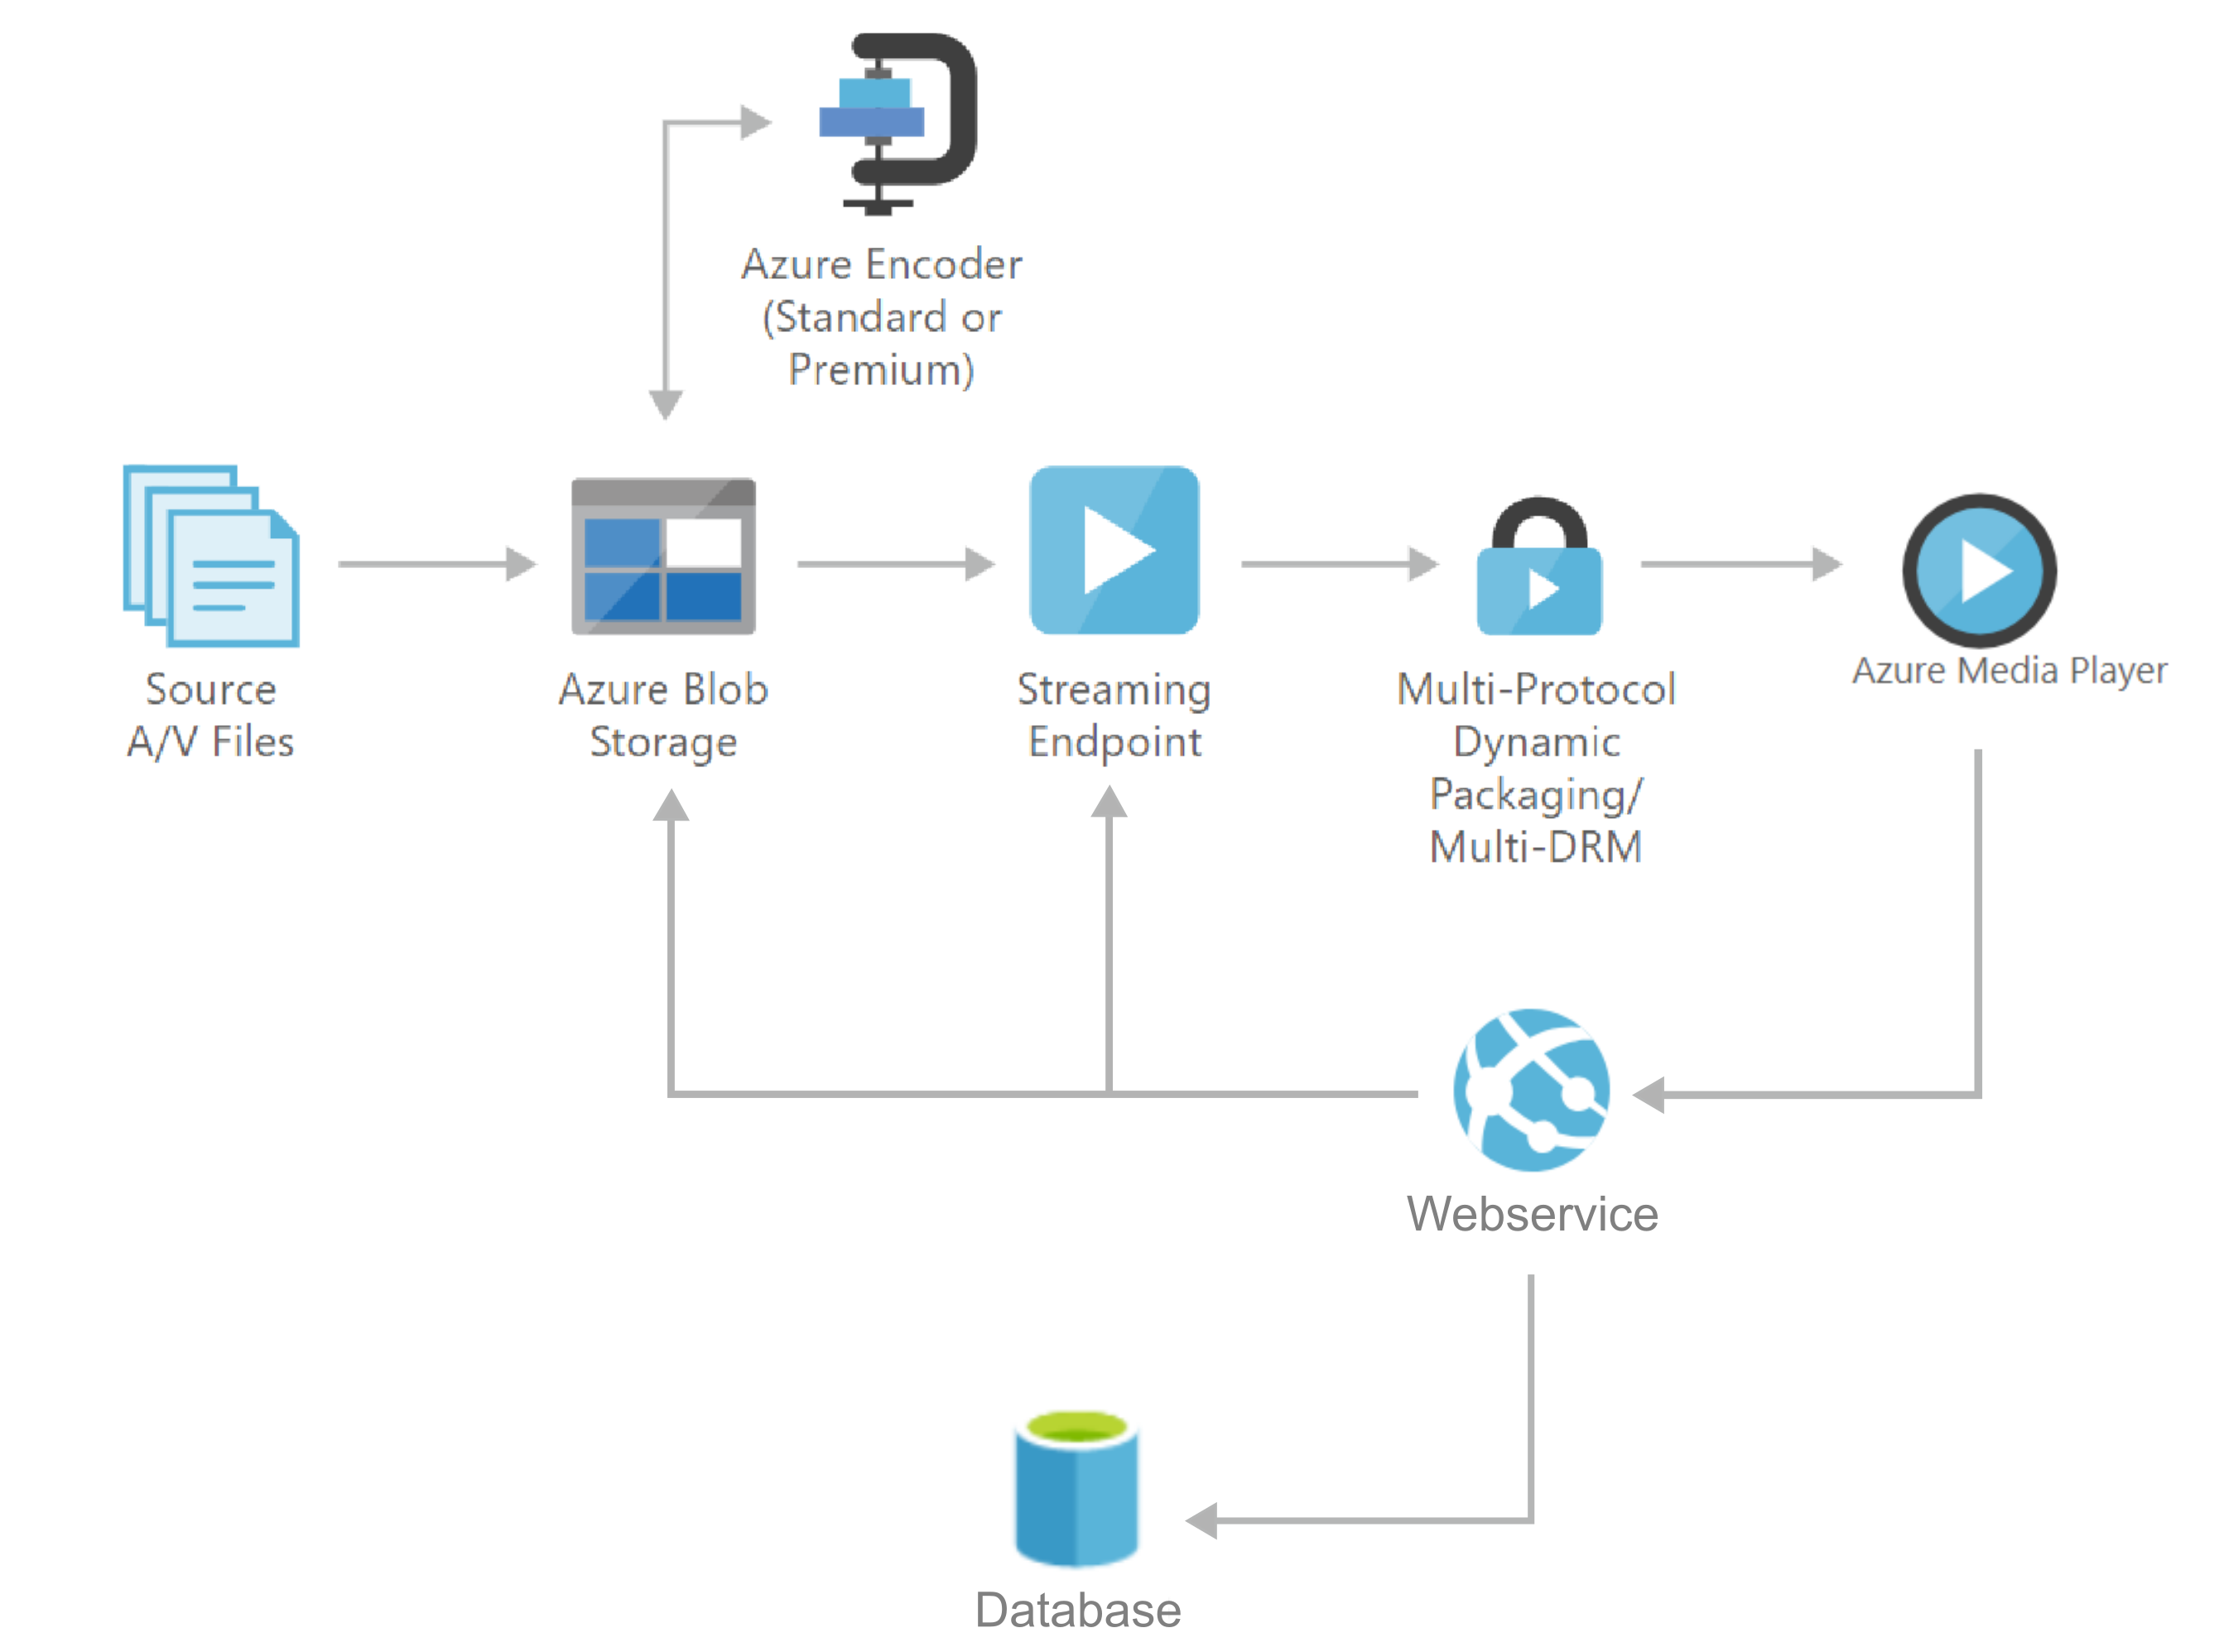
\includegraphics[width=1\textwidth, height=240px]{ressources/architecture_new.png}
    \caption{Modificated implementation of Microsofts VoD architecture}
    \label{fig:arch_new}
  \end{figure}
% ACuch benötigt laut config.js:  Azure ActiveDirectory (aad) id, secret, tenantID
% das hier?    https://docs.microsoft.com/de-de/azure/active-directory/develop/howto-create-service-principal-portal#create-an-azure-active-directory-application
% jap, steht in depl-script, auskommentiert. einmalige ausführung

Using Media Services results in a \textit{two-tier} server-architecture, in which the NodeJS-powered AppService has the end-user's devices as clients. The webserver itself is a client to the Azure Media Services Backend, requesting Encoding- and Streaming-Tasks by submitting \textit{Jobs}. This is also for security reasons, as Media Services uses a separate account-system with it's own credentials, generated by Microsoft. Those are confidential and must not be exposed to end-users. CORS (Cross Origin Resource Sharing) must be enabled for the Storage Account. 

The cloud components used scale completly automatic when needed. The NodeJS AppService is configurated to scale along the workload of the CPU resulting in creating another instance of the service. This happens once the defined threshold is reached. Incoming requests will automaticly distributed by Azure. The database behaves in the same way, scaling up and down when needed depending on the used price tier.